The figure~\ref{fig:scenario} illustrates our data integration metamodel.
The \textsl{Multi-Cloud} is configured as a set of \textsl{Cloud Infrastructures}. \textsl{Data producers} and \textsl{data consumers} subscribe to \textsl{cloud infrastructures}. 
Their subscription credentials are illustrated thanks to a \textsl{SLA} (\textsl{Consumer SLA} or \textsl{Producer SLA}) defining what the \textsl{cloud infrastructure} offers to them through their subscription. 
\textsl{Data} are provided and consumed by \textsl{Data Producers} and \textsl{Data Consumers}, respectively.

\begin{figure}[th!]
\center
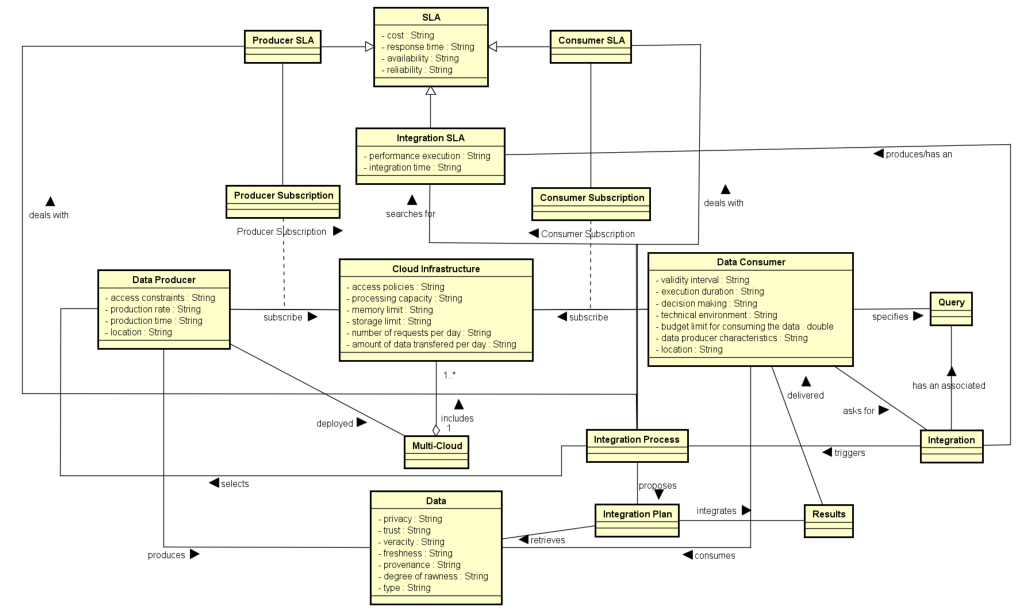
\includegraphics[scale=0.50]{metamodel.pdf}
\caption{Data integration metamodel}\label{fig:scenario}
\end{figure}

We propose a data integration meta-process in order to achieve quality and efficiency in the integration. 
Figure~\ref{fig:metaprocess} shows the meta-process composed by three macro-steps (query management, SLA management and query rewriting) which take into account the four principal dimensions (\textsl{Data consumer}, \textsl{Data Producer}, \textsl{Cloud Infrastructure} and \textsl{Data}) described in the metamodel.
The meta-process steps define a group of activities used in the data integration process.
The meta-process workflow can be seen as follows: \textit{first}, query management activities are performed to define the user query and preferences; \textit{second}, SLA management activities are executed to search and reuse previous SLAs used on integration (what we call \textsl{integration SLA}), and to create a new \textsl{integration SLA} for the current request; \textit{third}, query rewriting activities (as we partially described in~\cite{carvalho2016}) are proceeded to search and filter \textsl{data producers}, to generate and execute the integration plan, and to compute results; \textit{finally}, other SLA management activities take place to enforce the SLA associated to the involved services, and to update and store the final \textsl{integration SLA}. 

\begin{figure}[h!]
\center
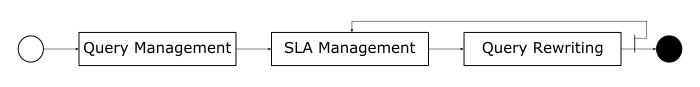
\includegraphics[scale=0.50]{meta-process.png}
\caption{Data integration meta-process}\label{fig:metaprocess}
\end{figure}

The activities defined in our meta-process bring challenges to our research as discussed in the next lines:
\begin{enumerate}
\item \underline{Search and reuse of previous \textsl{integration SLA}}. The new kind of SLA what we call \textsl{integration SLA} should be designed to include the information concerning the user requirements and preferences, the user query and the services used in the integration that satisfy the requirements, preferences and constraints imposed by the multi-cloud. Moreover, we must identify important information collected during the integration that should be saved in order to be reused in the next integration making the entire process more efficient. 
\item \underline{Query rewriting activities}. The query rewriting activities deal with a complex matching process of user requirement and preferences with constraints imposed by the context, and expressed in different SLAs. Furthermore, during the execution, it is also necessary to enforce the SLAs associated to the \textsl{data producers}. In this process, perhaps a given \textsl{producer} can out of resources for processing the request.
\item \underline{Computing results}. Retrieving, integrating and delivering are tasks that requires a large amount of resources and processing time. Thus, it is necessary to study a clever manner to make efficient the overall execution, and also there is an important decision making step while choosing the best cloud to proceed with the integration.
\end{enumerate}

%Taking into consideration at real-time the entities presented in our metamodel and our meta-process, we propose a SLA-based data integration process adapted to the multi-cloud below.
%%
%A users specifies a query according to his/her needs and requirements. In addition, he/she defines a set of preferences and associate them to the query. Given a query and user preferences, previous integration SLAs (that are associated to a previous integration) that matches with the actual query and preferences are searched. If a match is found, the information about this previous integration is reused and a new integration SLA is created using this information. On the other hand, if no match is found, a new integration SLA is created without any previous information. Then, a set of query rewriting activities are performed to generate the execution plan. Results are computed and the integration SLA is updated and stored to be used in a next integration request. The query rewriting activities sub-process include (i) searching for data producers that can produce an answer to the query;  (ii) filtering data producers according to the user preferences, to the consumer SLAs and to the producer SLAs. This means it is necessary to verify if the data producer is out of resources or not, and if the consumer has enough resources to process the data provided by the producer; (iii) generating the execution plan according to the SLAs; (iv) enforcing the SLAs associated to the involved services; and (v) executing the integration plan. Computing results sub-process retrieves data, integrates results and deliver them.
%

%\textsc{\begin{figure}[h!]
%\center
%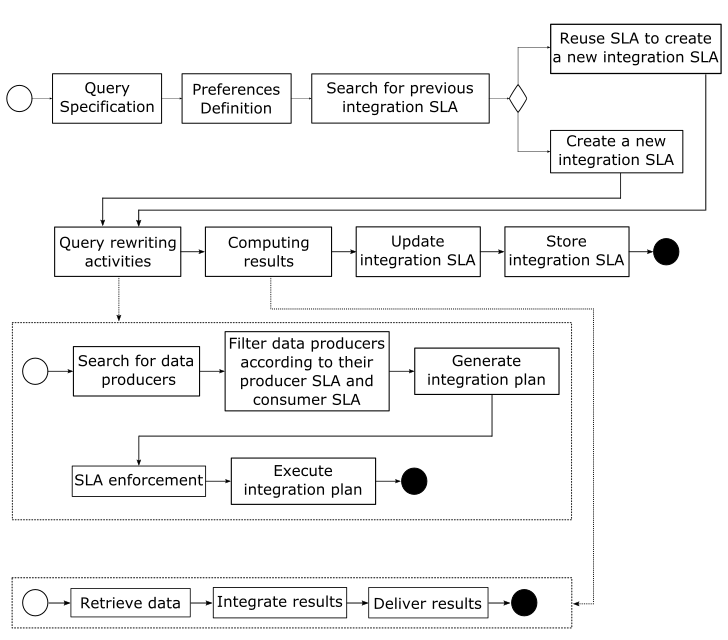
\includegraphics[scale=0.50]{process.png}
%\caption{Data integration process}\label{fig:process}
%\end{figure}}


%Given a user \textit{query}, a set of associated user \textit{preferences} and \textsl{Data Consumers}:
%\\
%\textbf{\underline{SLA derivation}}. In this step, we compute what we call an \textsl{integration SLA} that matches user' integration requirements (including quality constraints and data requirements) with the \textsl{SLA}'s provided by \textsl{data producers}, given a specific user cloud subscription. The user may have general requirements depending on the context he/she wants to integrate his/her data such as economic cost, bandwidth limit, free services, and storage and processing limits. The \textit{SLA derivation} is the big challenge while dealing with SLAs and particularly for adding quality dimensions to data integration. Furthermore, the \textsl{integration SLA} guides the query evaluation, and the way results are computed and delivered. \\
%\textbf{\underline{Filtering data services}}. The \textsl{integration SLA} is used (i)
%to filter previous \textsl{integration SLA} derived for a similar request in order to reuse results; or (ii) to filter possible \textsl{data producers} that can be used for answering the query. \\ %The SLA exported by a selected \textit{cloud service} should satisfy the user \textit{preferences}. \\
%\textbf{\underline{Query rewriting}}. Given a set of \textit{data producers} that can
%potentially provide data for integrating the query result, a set of service compositions is generated according to the \textsl{integration SLA} and the agreed \textsl{Producer SLA} of each \textsl{data producer}. \\
%\textbf{\underline{Integrating a query result}}. The service compositions are
%executed with services from one or several clouds where the user has a
%subscription.
%The execution cost of service compositions must fulfill the \textsl{integration
%SLA}. The clouds resources needed by the user to execute the composition and how
%to use them is decided taking in consideration the economic cost determined by
%the data to be transferred, the number of external calls to services, data storage and delivery cost.

%The algorithm 1 describes in general lines our approach which integrate data
%from multi-cloud environments considering quality aspects.
%%
%As input, we consider (1) a user query $Q$; (2) a set of user preferences $P$;
%(3) a user cloud subscription $C$; (4) a set of previous \textit{integrated SLA}
%$\bigSLA$, obtained from a local register; (5) a set of \textit{data services}
%$DS$; (6) a set of \textit{data processing services} $DPS$; and (7) a set of \textit{cloud providers} $CP$. As output, the integration results $IR$ is delivered to the user while fulfilling her preferences and cloud subscription.
%%
 
%The approach begins looking for previous \textit{integrated SLAs} in our
%local registry. From each \textit{integrated SLA} we verify if it matches
%the user' query and preferences (lines 2 - 6), and adding them to the set $pI$ (line 4).
%%
%If previous \textit{integrated SLA} matches (line 7), the one that
%partially matches with the user preferences is selected (line 8).
%%
%Then, a new \textit{integrated SLA} is computed for user query based on the
%previous \textit{integrated SLA}, her preferences and cloud subscription (line 9).
%%
%The service compositions produced to a previous query is reused based its \textit{integrated SLA} ($sI$). 
%%
%Otherwise, a new \textit{integrated SLA} is created to user request given the query, her preferences and cloud subscription (line 11). 
%%
%The SLA information of $\mathit{DS}$ and $\mathit{DPS}$ is extracted and included in the set of \bigS (line 12). 
%%
%This new \textit{integrated SLA} is updated by calling the \textit{Rhone} procedure (line 13). 
%%
%The \textit{Rhone} is responsible of (i) selecting \textit{data services} (in $DS$) and \textit{data processing services} (in $DPS$) which satisfy the user preferences based on their SLAs; and (ii) producing service compositions that completely match with the query and fulfill the user preferences. 
%%
%Finally, the integration results ($IR$) are produced and delivered to the user considering her cloud subscription. 
%%
%Note that while executing compositions, it is necessary to satisfy the user requirements and cloud subscription, and also to dynamically update the \textit{integrated SLA} adding the information of contracts that were established to allow the integration. 
%%
%Finally, the \textit{integrated SLA} is stored in our registry to be used in a next query.   
%
%\begin{algorithm} 
%%\small
%\caption{ - SLA-based data integration}
%\label{qualityBasedAlgorithm}
%\begin{algorithmic}[1]
%\REQUIRE Query ($Q$), user preferences ($P$), user cloud subscriptions ($C$), a
%set of \textit{data services} ($\mathit{DS}$) and \textit{data processing services} ($\mathit{DPS}$) and a set of previous \textit{integrated SLA} ($\bigSLA$).
%\ENSURE Integration results delivered considering the user cloud subscription.
%%\STATE \textbf{function} $\mathit{SelectCandidateServices} (Q, \bigS)$
%%\STATE let $\bigSLA$ be a set of previous integrated SLA
%\STATE $pI \leftarrow \emptyset$
%\FORALL  {$SLA_{i}$ in $\bigSLA$}
%	\IF {$\mathit{macthes(Q, P, SLA_{i})}$}
%		\STATE $pI \leftarrow pI \cup \lbrace SLA_{i} \rbrace$		
%%		\FORALL  {$A_{j}$ in $S_{i}$}
%%			\IF {$Q.\mathit{notContains(A_{i})}$}
%%				\STATE $b \leftarrow \mathit{false}$	
%%				\STATE $\mathit{break}$
%%			\ENDIF
%%		\ENDFOR
%%		\IF {$b = true$}
%%			\STATE $\bigLS \leftarrow \bigLS \cup \lbrace S_{i} \rbrace$	
%%		\ENDIF
%	\ENDIF
%\ENDFOR
%\IF {$pI \neq \emptyset$}
%	\STATE $sI \leftarrow chooseBest(P, pI)$
%	\STATE $newSLA_{i} \leftarrow deriveSLA(sI, P, C)$
%%	\FORALL  {$SLA_{i}$ in $pI$}
%%		\STATE $sI \leftarrow choose(P,)$
%%	\ENDFOR
%\ELSE
%	\STATE $newSLA_{i} \leftarrow deriveSLA(Q, P, C)$
%	\STATE $\bigS \leftarrow extract(\mathit{DS}, \mathit{DPS})$
%	\STATE $newSLA_{i} \leftarrow updateSLA(Rhone(Q, \bigS))$
%\ENDIF
%\STATE $IR \leftarrow execute(newSLA_{i})$
%\STATE \textbf{return} $IR$
%\STATE \textbf{end function}
%\end{algorithmic}
%\end{algorithm} 

%\subsection{SLA-based query rewriting algorithm}
%To serve a proof of concept to our approach, we develop a query
%rewriting algorithm which is guided by users' integration requirements and
%service level agreements exported by different data services and cloud
%providers. Researches have refered to data integration as a service composition problem
%in which given a query the objective is to lookup and compose data services that
%can contribute to produce a result. Currently, we have formalized and developed a rewriting
%algorithm that considers user preferences and services' quality aspects while
%selecting services and producing rewritings called \textit{Rhone} (See algorithm
%\ref{algo-rhone}, invoked in the algorithm 1, line 12).
%The \textit{Rhone} algorithm consists in four macro steps: 
%\\
%\textbf{\underline{Selecting data services}}. The \textit{Rhone} looks for
%\textit{data services} (line 2) that can contribute to answer the query while
%satisfying the user' preferences; \\
%\textbf{\underline{Building candidate service descriptions}}. A candidate
%service description (CSD) describes how a \textit{data service} can contribute to answer the query. CSD maps a \textit{data service} (including its variables) to the entire query or part of it. For all selected services, the \textit{Rhone} tries to build CSDs when the mapping of variables is possible (line
%3). \\
%\textbf{\underline{Combining CSDs}}. All CSDs are combined (line 4) producing a
%list of CSD combinations. Each combination can be a rewriting of the query. \\
%\textbf{\underline{Producing rewritings}}. Each list of CSDs is checked in order
%to verify whether it is a rewriting of the query or not (line 9). To be a
%valid rewriting, it is forbidden to have CSDs covering the same part of the query.
%Rewritings are produced while the user' requirements are being respected (lines 6-14).
%%
%The originality of our algorithm concerns the functions ~\!\tqI{}, ~\!\tqT{} and ~\!\tqS{}.     
%They are responsible to initialize, check and increment user preferences
%associated to some aggregation like user constraints (total cost). This means
%that these preferences are initialized (line 6), and for each element in the CSD list they are incremented (line 11), and rewritings are produced while they are respected (line 8).  The result of this step is the list of valid rewritings of the query (line 14).
%
%\begin{algorithm}[h!]
%\small
%\caption{ - \textit{Rhone}}
%\label{algo-rhone}
%\begin{algorithmic}[1]
%\REQUIRE A query $Q$, a set of user preferences, and a set of concrete services $\bigS$.
%\ENSURE A set of rewritings $R$ that matches with the query and fulfill the user preferences.
%\STATE \textbf{function} $\mathit{Rhone} (Q, \bigS)$
% \STATE  $\bigLS \leftarrow \mathit{SelectCandidateServices}(Q, \bigS)$ \label{rhone:buildPCD}
% \STATE  $\bigLCSD \leftarrow CreateCSDs(Q, \bigLS)$
% \STATE  $I \leftarrow CombineCSDs(\bigLCSD)$
% \STATE $R\leftarrow \emptyset$
% \STATE ~\!\tqI{\agg{Q}} 
%    \STATE $p \leftarrow I.next()$
%    \WHILE {$p\ \neq\ \emptyset$ \AND ~\!\tqT{\agg{Q}}} 
%      \IF {\textit{isRewriting}$(Q, p)$}
%  \STATE $R\leftarrow R\,\cup \mathit{Rewriting}(p)$
%  \STATE ~\!\tqS{\agg{Q}}
%   \ENDIF
%      \STATE $p \leftarrow I.\mathit{next}()$
% \ENDWHILE
%    \STATE \textbf{return} $R$
%\STATE \textbf{end function}
%\end{algorithmic}
%\end{algorithm}
%
%To serve as a proof of concept to our approach, we intend to develop a query
%rewriting algorithm which is guided by users' integration requirements and
%service level agreements exported by different data services and cloud
%providers. The query rewriting is an important issue in data integration. In
%cloud computing, researches have refereed to it as a service composition problem
%in which given a query the objective is to lookup and compose data services that
%can contribute to produce a result. \cite{Barhamgi2010} proposed a query
%rewriting approach which processes queries on data provider services.
%\cite{Benouaret2011} introduced a service composition framework to answer
%preference queries. Two algorithms inspired on~\cite{Barhamgi2010} are presented
%to rank the best rewritings based on previously computed scores. \cite{ba2014}
%extended \cite{Umberto} and presented an refinement algorithm that produces and
%order rewritings according to user preferences and scores. In general, these
%works share the same performance problem depending on the size of the query and
%on the number of available services. Furthermore, they do not take into
%consideration user's integration requirements what can lead to produce
%rewritings that are not satisfactory to the user in terms of quality
%requirements and cost. Currently, we have formalized and developed a rewriting
%algorithm that considers user preferences and services' quality aspects while
%selecting services and producing rewritings called \textit{Rhone} (Invoked in the algorithm 1, line 12).                     